\section{Introduction}

Reinforcement learning has become a central algorithmic driver of recent advances in large language models, substantially enhancing their ability to solve complex tasks and enabling a new class of reasoning-focused models such as OpenAI o1 \citep{Openai-O1}, DeepSeek R1 \citep{Deepseek-R1}, and Qwen3 \citep{Qwen3}. 
Yet, scaling RL for reasoning over long horizons remains fragile: \textbf{stable optimization can still yield unstable generalization}.

While the community has extensively addressed system-level instabilities, such as the training-inference mismatch \citep{GSPO, IcePop, XiaomiR3, MiniRL}---an architectural inconsistency that disrupts optimization \citep{TIS, SpeedStability}---we focus on a more fundamental algorithmic failure: \textit{\textbf{over-optimization}} \citep{gao2023scaling}.
As illustrated in Fig.~\ref{fig:teaser}, we observe a distinctive \textit{reward--validation gap}: training reward (answer correctness) improves steadily, yet validation performance decouples and degrades.
In this regime, stable reward curves can even be a warning sign rather than a reassurance.
This phenomenon, echoed in recent works \citep{clipfairly, zhang2025gepo}, indicates a breakdown in generalization rather than an optimization collapse.

% Despite these successes, scaling RL training over long horizons faces significant stability hurdles.
% The community has extensively addressed the \textit{\textbf{training-inference mismatch}}, an issue arising from discrepancies between high-performance inference engines and distributed training backends \citep{TIS, SpeedStability}.
% Such architectural inconsistencies can lead to numerical divergence or even model collapse \citep{TIS}, especially within mixture-of-experts (MoE) models \citep{IcePop}.
% While various remedies exist for these mechanical issues \citep{TIS, GSPO, XiaomiR3, MiniRL}, a more insidious challenge remains: the \textbf{\textit{over-optimization}} problem \citep{gao2023scaling}.
% This algorithmic instability manifests as a distinct \textit{reward-validation gap}:
% As illustrated in Fig.~\ref{fig:teaser}, we observe that training rewards (answer correctness) rise steadily, indicating that the optimization itself is stable, yet validation performance decouples and declines after an initial ascent.
% This phenomenon, echoed in recent works \citep{clipfairly, zhang2025gepo}, highlights a failure of generalization rather than optimization.

\begin{figure}[t]
    \centering
    \begin{subfigure}[b]{0.38\linewidth}
        \centering
        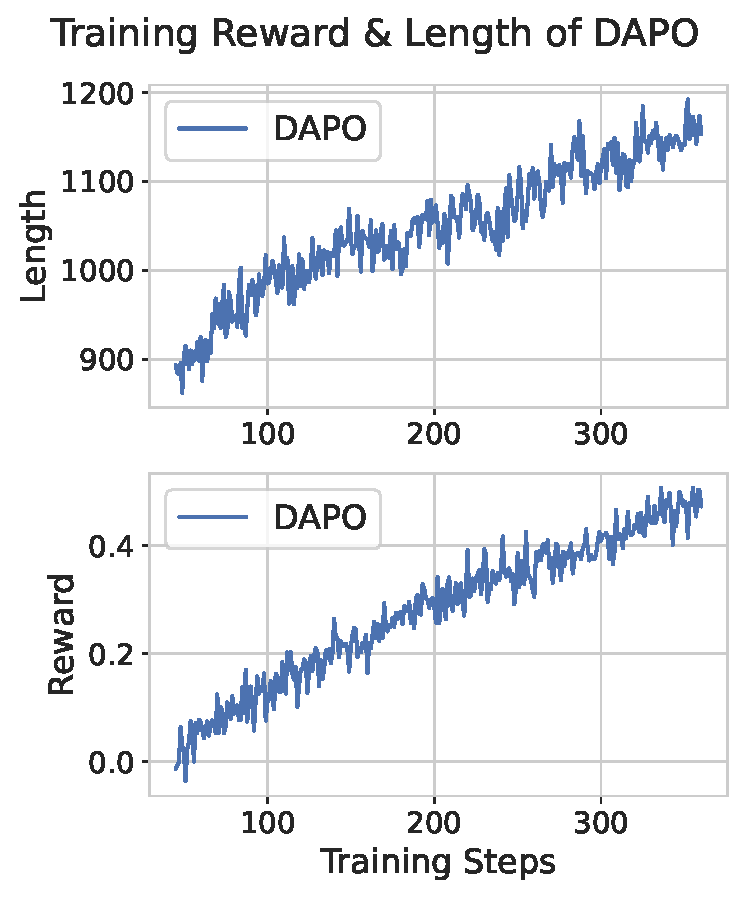
\includegraphics[width=\linewidth]{figs/teaser_metrics.pdf}
        \caption{Training behaviors}
        \label{fig:teaser_reward}
    \end{subfigure}
    \hfill
    \begin{subfigure}[b]{0.6\linewidth}
        \centering
        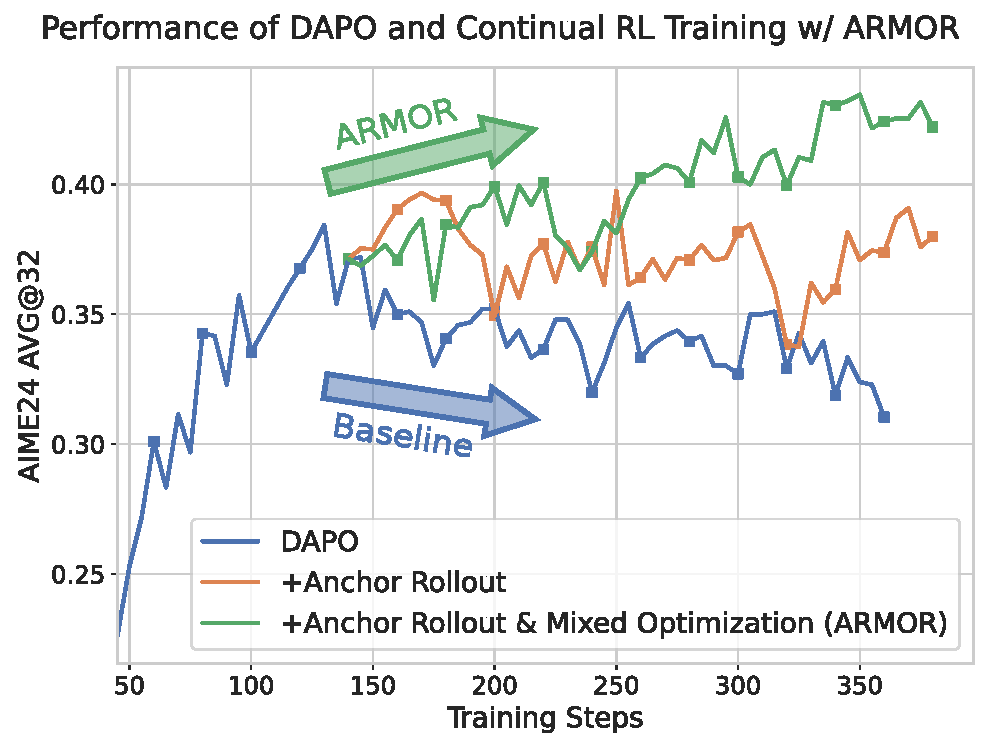
\includegraphics[width=\linewidth]{figs/teaser_acc.pdf}
        \caption{Validation score (AIME24)}
        \label{fig:teaser_perf}
    \end{subfigure}
    \caption{Illustration of the over-optimization issue and the efficacy of ARMOR (on Qwen2.5-Math-7B).
    (a) Training reward and response length steadily rise, indicating stable optimization. 
    (b) However, validation performance reveals a critical generalization failure: the \textcolor{myblue}{baseline} performance degrades after an initial ascent. 
    By integrating \textcolor{myorange}{anchor rollout} to stabilize the sample distribution and mixed optimization to enhance exploration, \textcolor{mygreen}{ARMOR} prevents degradation and sustains continuous performance gains.}
    \label{fig:teaser}
\end{figure}

Crucially, this failure differs from the classical form of \textit{reward hacking} that arises from a discrepancy between a proxy reward and the true evaluation metric \citep{weng2024rewardhack}.
In reasoning tasks with \textit{verifiable rewards} \citep{tulu-RLVR}, the reward signal remains consistent across training and validation.
Nevertheless, the model still tends to over-optimize solution patterns that yield high rewards on seen data but fail to generalize, necessitating algorithmic intervention beyond simple reward correction \citep{ding2025fapo}.
% This suggests that the instability arises from the policy's tendency to latch onto spurious correlations in the training set, necessitating algorithmic intervention beyond simple reward correction.
% As the policy iterates, the on-policy rollout distribution progressively concentrates on a narrow set of high-reward patterns. 

Unfortunately, we find the standard algorithmic defense, reverse KL regularization \citep{ouyang2022training, gao2023scaling}, is often insufficient in this regime due to two intrinsic limitations (Fig.~\ref{fig:kl_explain}): 
\textbf{(1) Mode-seeking nature (Instability):} Reverse KL only penalizes the policy for generating samples \emph{unlikely} under the reference. Consequently, the policy can still collapse onto a narrow subset of ``shortcut'' patterns without incurring a high penalty, losing the diversity of the reference %original 
distribution \citep{beyondkl, klcollapse}.
\textbf{(2) Uniform penalty (Stagnation):} By indiscriminately suppressing deviation from the reference, the KL term dampens the exploration required to discover superior reasoning paths that lie beyond the initial distribution.

%Importantly, this failure is not classical \textit{reward hacking} driven by exploitable proxy rewards \citep{weng2024rewardhack}.
% Unlike typical reward hacking driven by exploitable proxy models \citep{weng2024rewardhack}, reasoning tasks here rely on \textit{verifiable rewards} \citep{tulu-RLVR} where the evaluation mechanism remains consistent across training and validation.
% Despite such consistency, models still drift toward over-optimizing specific training shortcuts, necessitating algorithmic intervention beyond simple reward design.
% Despite this objective supervision, the divergence between rising training rewards and decreasing validation performance points to an over-optimization of training shortcuts that requires algorithmic intervention.
% Although this divergence is often broadly categorized as reward hacking \citep{weng2024rewardhack, gao2023scaling}, it is more nuanced in the context of reasoning tasks with \textit{verifiable rewards} \citep{tulu-RLVR}.
% Even under strict answer correctness supervision, models tend to \textbf{\textit{over-optimize}} specific training heuristics or shortcuts rather than acquiring robust, generalizable reasoning patterns.
% Consequently, mitigating this over-optimization is a prerequisite for unlocking the next stage of RL scaling.
% Unfortunately, we find the standard algorithmic defense, reverse KL regularization \citep{ouyang2022training}, is often insufficient in this regime \citep{gao2023scaling}.
% However, standard reverse KL regularization, the conventional defense against such over-optimization \citep{ouyang2022training}, is often insufficient in this regime \citep{gao2023scaling}.
% Our analysis suggests that such simple penalty terms fail because they: 
% \begin{enumerate}[left=0.5em, topsep=0pt, itemsep=0pt]
% \item [(1)] lack direct exposure to \emph{high-quality reference samples};
% % \item [(2)] can inadvertently push the optimization into suboptimal directions by \emph{penalizing deviations too broadly}.
% \end{enumerate}

To address these limitations, we propose \textbf{ARMOR ({\ul A}nchor {\ul R}ollout and {\ul M}ixed {\ul O}ptimization for {\ul R}L)}, a framework that shifts focus from passive loss penalty to active sample stabilization. Our approach comprises two key components, each targeting a specific failure mode of standard KL:
\begin{enumerate}[left=0.5em, topsep=2pt, itemsep=2pt]
\item [(1)] \textbf{Anchor Rollout (Addressing Instability)}: Instead of relying on a passive KL loss to retain distribution modes, we \emph{actively} inject off-policy samples from the reference policy during rollout. 
This acts as an explicit ``anchor'' forcing the model to recall and preserve established generalizable solution patterns.
\item [(2)] \textbf{Mixed optimization (Addressing Stagnation)}: We remove the auxiliary penalty term and instead optimize a mixed policy $\alpha\cdot \pi_\theta + (1-\alpha) \cdot \pi_\mathrm{ref}$, to principally align the optimization target and data distribution.
Crucially, this mixture constructs an adaptive trust region \citep{PPO} that permits controlled exploration without the suppressive effect of a uniform penalty.
\end{enumerate}
As visualized in Fig.~\ref{fig:teaser_perf}, ARMOR effectively bridges the generalization gap, maintaining superior validation performance compared to the degraded baseline.
We validate these benefits through extensive experiments across different base models (\eg Qwen2.5-Math-7B, Qwen3-8B-Base) and RL algorithms (\eg DAPO \citep{DAPO}, QAE \citep{QAE}). 
The results on various reasoning benchmarks confirm that our framework not only secures prolonged training stability but also unlocks continuous performance gains.

% \begin{enumerate}[left=0.5em, topsep=0pt, itemsep=0pt]
% \item [(1)] \textbf{Anchor rollout}: During rollout, we inject off-policy samples generated by reference policy $\pi_{\mathrm{ref}}$, acting as an explicit regularization ``anchor'' preventing the model from forgetting established generalizable solutions.
% \item [(2)] \textbf{Mixed optimization}: We reformulate the objective to optimize a mixed policy $\alpha\cdot \pi_\theta + (1-\alpha) \cdot \pi_\mathrm{ref}$. 
% This allows for a more controlled exploration space (e.g., via broadened clip ranges) without introducing auxiliary loss penalties that suppress exploration.
% \end{enumerate}